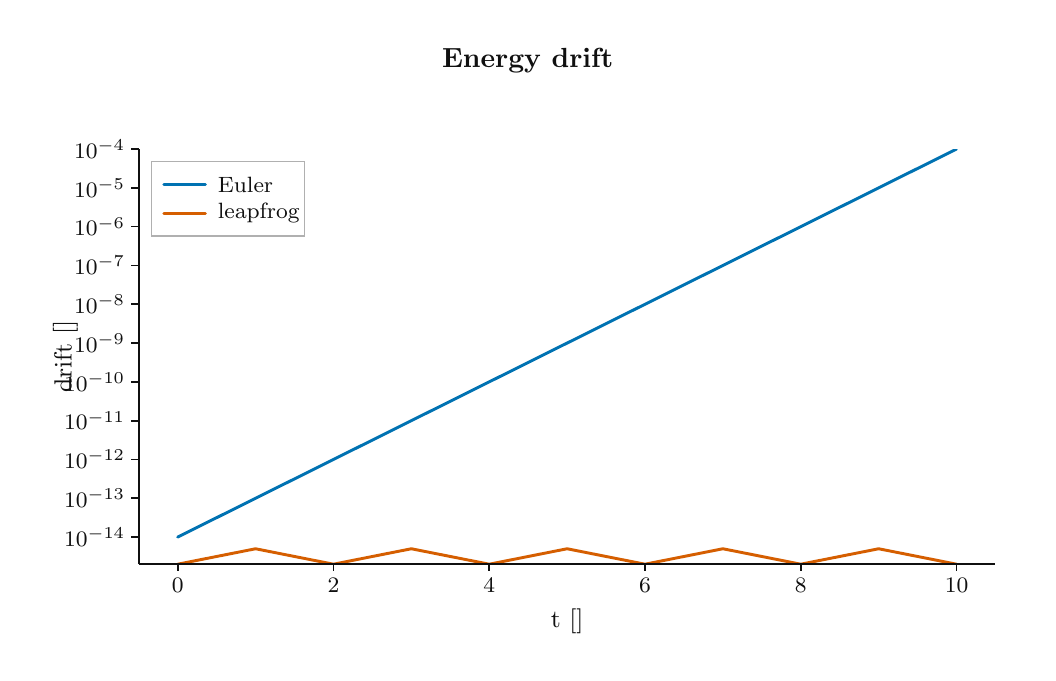
\begin{tikzpicture}[every node/.style={inner sep=0bp,outer sep=0bp}]
  \definecolor{qcA}{rgb}{1,1,1}
  \definecolor{qcB}{rgb}{0.062745,0.062745,0.062745}
  \definecolor{qcC}{rgb}{0,0.447059,0.698039}
  \definecolor{qcD}{rgb}{0.835294,0.368627,0}
  \definecolor{qcE}{rgb}{0.690196,0.690196,0.690196}
  \useasboundingbox (0bp,0bp) rectangle (360bp,225bp);
  % marey-key: figure
  \path[fill=qcA] (0bp,0bp) -- (360bp,0bp) -- (360bp,225bp) -- (0bp,225bp) -- cycle;
  % marey-role: annotation -- Energy drift
  \node[anchor=north,text=qcB,font=\bfseries\fontsize{10}{12}\selectfont] at (180bp,217.5bp) {Energy drift};
  % marey-key: figure/panel-0-0
  % marey-role: other:panel -- panel
  % marey-data: row = 0
  % marey-data: col = 0
  % marey-data: layers = 2
  % marey-data: x-tick-rule = all
  % marey-data: y-tick-rule = all
  \begin{scope}
    \clip (39.987bp,31.85bp) -- (348.408bp,31.85bp) -- (348.408bp,181.3bp) -- (39.987bp,181.3bp) -- cycle;
    % marey-key: figure/panel-0-0/layer-0
    % marey-role: series -- Euler
    % marey-data: series = Euler
    % marey-data: points = 11
    \path[draw=qcC,line width=1.05bp,line cap=round,line join=round] (54.006bp,41.614bp) -- (82.044bp,55.582bp) -- (110.083bp,69.551bp) -- (138.121bp,83.52bp) -- (166.159bp,97.488bp) -- (194.197bp,111.457bp) -- (222.236bp,125.425bp) -- (250.274bp,139.394bp) -- (278.312bp,153.363bp) -- (306.35bp,167.331bp) -- (334.389bp,181.3bp);
    % marey-key: figure/panel-0-0/layer-1
    % marey-role: series -- leapfrog
    % marey-data: series = leapfrog
    % marey-data: points = 11
    \path[draw=qcD,line width=1.05bp,line cap=round,line join=round] (54.006bp,31.85bp) -- (82.044bp,37.409bp) -- (110.083bp,31.85bp) -- (138.121bp,37.409bp) -- (166.159bp,31.85bp) -- (194.197bp,37.409bp) -- (222.236bp,31.85bp) -- (250.274bp,37.409bp) -- (278.312bp,31.85bp) -- (306.35bp,37.409bp) -- (334.389bp,31.85bp);
  \end{scope}
  % marey-key: figure/panel-0-0/axis-x
  % marey-role: axis -- t [s]
  % marey-data: side = bottom
  % marey-data: unit = s
  % marey-data: prefix =
  % marey-data: ticks = 6
  % marey-data: tick-rule = all
  \path[draw=qcB,line width=0.6bp] (39.987bp,31.85bp) -- (348.408bp,31.85bp);
  \path[draw=qcB,line width=0.6bp] (54.006bp,31.85bp) -- (54.006bp,29.225bp) (110.083bp,31.85bp) -- (110.083bp,29.225bp) (166.159bp,31.85bp) -- (166.159bp,29.225bp) (222.236bp,31.85bp) -- (222.236bp,29.225bp) (278.312bp,31.85bp) -- (278.312bp,29.225bp) (334.389bp,31.85bp) -- (334.389bp,29.225bp);
  \node[anchor=north,text=qcB,font=\fontsize{8}{9.6}\selectfont] at (54.006bp,26.975bp) {0};
  \node[anchor=north,text=qcB,font=\fontsize{8}{9.6}\selectfont] at (110.083bp,26.975bp) {2};
  \node[anchor=north,text=qcB,font=\fontsize{8}{9.6}\selectfont] at (166.159bp,26.975bp) {4};
  \node[anchor=north,text=qcB,font=\fontsize{8}{9.6}\selectfont] at (222.236bp,26.975bp) {6};
  \node[anchor=north,text=qcB,font=\fontsize{8}{9.6}\selectfont] at (278.312bp,26.975bp) {8};
  \node[anchor=north,text=qcB,font=\fontsize{8}{9.6}\selectfont] at (334.389bp,26.975bp) {10};
  \node[anchor=north,text=qcB,font=\fontsize{9}{10.8}\selectfont] at (194.197bp,15.825bp) {t [\qty{}{\second}]};
  % marey-key: figure/panel-0-0/axis-y
  % marey-role: axis -- drift [J]
  % marey-data: side = left
  % marey-data: unit = J
  % marey-data: prefix =
  % marey-data: ticks = 11
  % marey-data: tick-rule = all
  \path[draw=qcB,line width=0.6bp] (39.987bp,31.85bp) -- (39.987bp,181.3bp);
  \path[draw=qcB,line width=0.6bp] (39.987bp,41.614bp) -- (37.362bp,41.614bp) (39.987bp,55.582bp) -- (37.362bp,55.582bp) (39.987bp,69.551bp) -- (37.362bp,69.551bp) (39.987bp,83.52bp) -- (37.362bp,83.52bp) (39.987bp,97.488bp) -- (37.362bp,97.488bp) (39.987bp,111.457bp) -- (37.362bp,111.457bp) (39.987bp,125.425bp) -- (37.362bp,125.425bp) (39.987bp,139.394bp) -- (37.362bp,139.394bp) (39.987bp,153.363bp) -- (37.362bp,153.363bp) (39.987bp,167.331bp) -- (37.362bp,167.331bp) (39.987bp,181.3bp) -- (37.362bp,181.3bp);
  \node[anchor=east,text=qcB,font=\fontsize{8}{9.6}\selectfont] at (35.112bp,41.614bp) {$10^{-14}$};
  \node[anchor=east,text=qcB,font=\fontsize{8}{9.6}\selectfont] at (35.112bp,55.582bp) {$10^{-13}$};
  \node[anchor=east,text=qcB,font=\fontsize{8}{9.6}\selectfont] at (35.112bp,69.551bp) {$10^{-12}$};
  \node[anchor=east,text=qcB,font=\fontsize{8}{9.6}\selectfont] at (35.112bp,83.52bp) {$10^{-11}$};
  \node[anchor=east,text=qcB,font=\fontsize{8}{9.6}\selectfont] at (35.112bp,97.488bp) {$10^{-10}$};
  \node[anchor=east,text=qcB,font=\fontsize{8}{9.6}\selectfont] at (35.112bp,111.457bp) {$10^{-9}$};
  \node[anchor=east,text=qcB,font=\fontsize{8}{9.6}\selectfont] at (35.112bp,125.425bp) {$10^{-8}$};
  \node[anchor=east,text=qcB,font=\fontsize{8}{9.6}\selectfont] at (35.112bp,139.394bp) {$10^{-7}$};
  \node[anchor=east,text=qcB,font=\fontsize{8}{9.6}\selectfont] at (35.112bp,153.363bp) {$10^{-6}$};
  \node[anchor=east,text=qcB,font=\fontsize{8}{9.6}\selectfont] at (35.112bp,167.331bp) {$10^{-5}$};
  \node[anchor=east,text=qcB,font=\fontsize{8}{9.6}\selectfont] at (35.112bp,181.3bp) {$10^{-4}$};
  \node[anchor=base,text=qcB,rotate=90,font=\fontsize{9}{10.8}\selectfont] at (15.825bp,106.575bp) {drift [\qty{}{\joule}]};
  % marey-key: figure/panel-0-0/legend
  % marey-role: legend -- legend
  % marey-data: entries = 2
  \path[fill=qcA,fill opacity=0.85,draw=qcE,line width=0.45bp] (44.487bp,150bp) -- (99.579bp,150bp) -- (99.579bp,176.8bp) -- (44.487bp,176.8bp) -- cycle;
  % marey-role: other:legend-entry -- Euler
  % marey-data: series = Euler
  % marey-data: color = #0072b2
  \path[draw=qcC,line width=1.05bp,line cap=round] (48.987bp,168.6bp) -- (63.987bp,168.6bp);
  \node[anchor=west,text=qcB,font=\fontsize{8}{9.6}\selectfont] at (68.487bp,168.6bp) {Euler};
  % marey-role: other:legend-entry -- leapfrog
  % marey-data: series = leapfrog
  % marey-data: color = #d55e00
  \path[draw=qcD,line width=1.05bp,line cap=round] (48.987bp,158.2bp) -- (63.987bp,158.2bp);
  \node[anchor=west,text=qcB,font=\fontsize{8}{9.6}\selectfont] at (68.487bp,158.2bp) {leapfrog};
\end{tikzpicture}
